\chapter{预备知识与概念}
\label{chap1}
本章介绍基于编码的加密方案涉及到的有限域知识,编码知识等等。有限域理论是编码理论的一个重要数学基础,有限域上的元素,多项式更好的描述了码字在加解密中的计算过程,编码知识则是加密算法的理论依据,能够选择好性质的码是保证加密算法安全和高效的前提。

\section{有限域基础理论}
\begin{define}[有限域]
	在有限集合$\mathbf{F}$上定义了两个二元运算:加法 “$+$” 和乘法 “$\bullet$”,如果$(\mathbf{F}, +)$是交换群,$\mathbf{F}$的非零元素对乘法构成交换群,而且乘法对加法满足分配律,则称$(\mathbf{F}, +, \bullet)$是有限域,如果$\mathbf{F}$集合元素的个数为$q$,则记作$\mathbb{F}_q$或者$GF(q)$。简单起见,我们将二元域记作$\mathbb{F}$。
\end{define}

\begin{define}[本原元]
	一个数域$GF(q)$,具有最大阶的域元素为本原元,即本原元为$a$,则$a^d=1(mod~ q)$成立,其中$d=\psi(q)$,$\psi(q)$是欧拉函数。
\end{define}

\begin{define}[不可约多项式]
	有限域$\mathbb{F}$上定义的多项式集合$F[x]=\{f(x)|f(x)=a_nx^n + ... + a_1x + a_0,a_i \in \mathbb{F}, a_n \neq 0, n \geq 0\}$,$F[x]$中次数大于1的多项式$f(x)$不能写成两个低次多项式的乘积,称$f[x]$是$\mathbf{F}$上不可约多项式。
\end{define}

\begin{define}[极小多项式]
	设$\mathbb{F}_q$是一个含有$q$个元素的有限域,$\mathbb{F}_p$是$\mathbb{F}_q$的一个含有$p$个元素的子域,$\alpha \in \mathbb{F}_q$。$\mathbb{F}_p$上的以$\alpha$为根,首项系数为$1$,并且次数最低的多项式称为$\alpha$在$\mathbb{F}_p$上的极小多项式。这里$1$是$\mathbb{F}_p$的单位元。
\end{define}

\begin{define}[本原多项式]
	设$\mathbb{F}_(q^n)$是一个含有$q^n$个元素的有限域,$\mathbb{F}_q$是$\mathbb{F}_(q^n)$的一个含有$q$个元素的子域。设$\alpha \in \mathbb{F}_(q^n)$为$\mathbb{F}_(q^n)$的一个本原元。$\alpha$在$\mathbb{F}_q$上的极小多项式称为$\mathbb{F}_q$上的一个本原多项式。
\end{define}

\section{编码基础知识}
基于编码的加密方案的设计,需要考虑编码理论的相关定理,码的性质,纠错能力影响因素等,本小节做基本的概念介绍。在本文中介绍编码理论我们集中在二元域$\mathbb{F} = GF(2)$上。

解密过程中,译码的表现是重中之重。编码理论实际上就是对含有噪声的信道上通信的研究,码字经过信道传输后,由于噪声的存在,会发生一定概率的错误,使得发送端和接收端的码字不相等,我们通常在二元对称信道模型上考虑译码情况。

\begin{figure}[H]
	\centering
	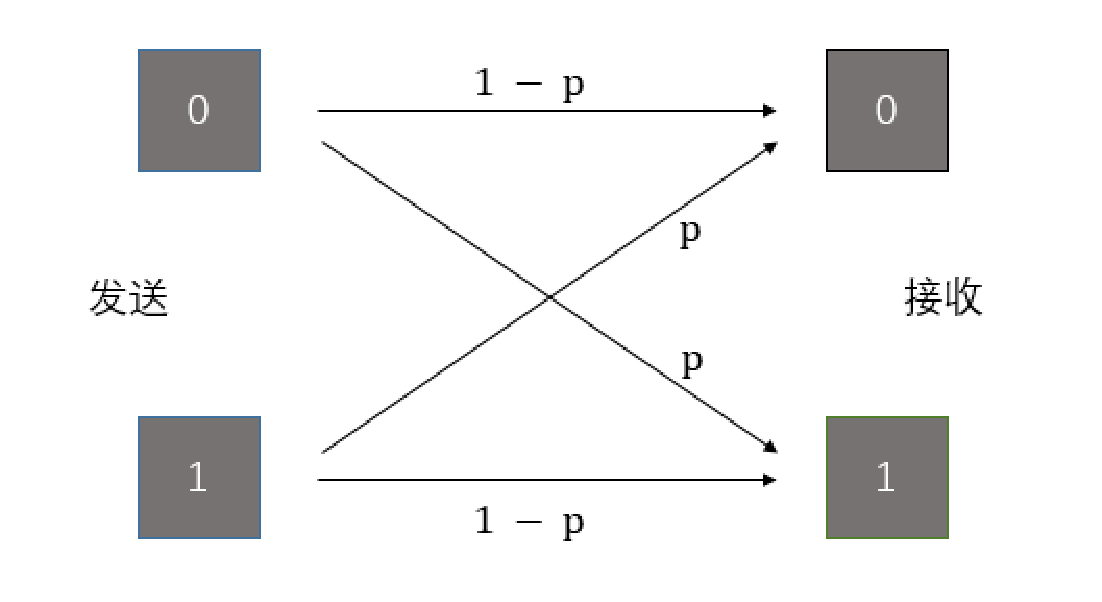
\includegraphics[width=12 cm]{fig/binarysymmetricchannel.pdf}
	\caption{二元对称信道} %\vspace*{-1.0cm}
	\label{fig:binarysymmetricchannel_pdf}
\end{figure}

\begin{define}[汉明重量与汉明距离]
	一个码字$\textbf{x}$的汉明距离定义为码字本身含有的非零位的个数,并表示为:$wt(\textbf{x})$。汉明距离指的是两个长度相同的码字$\textbf{x}, \textbf{y}$之间,位不同的总数,一般记作:$dist(\textbf{x}, \textbf{y})$。可以看出,$dist(\textbf{x}, \textbf{y}) = wt(\textbf{x} - \textbf{y})$。
\end{define}

\begin{define}[线性码]
	向量空间$\mathbb{F}^n$上的一个$k$维子空间定义为$[n, k]$线性码,记作:$\mathcal{C}$。另外,线性码$\mathcal{C}$的最小距离指的是,线性码中任意两个不同的码字之间的最小汉明距离,记作$d$。我们可以用$[n, k, d]$来表示最小距离为$d$的线性码$\mathcal{C}$,且最大纠错能力为$\lfloor(d - 1)\rfloor/2$。
\end{define}

\begin{define}[生成矩阵与校验矩阵]
	线性码$\mathcal{C}$的生成矩阵是指一个$k \times n$的矩阵$G$,$G$的行可以构成线性码$\mathcal{C}$的基。也就是说由矩阵$G$的行可以线性组合成线性码$\mathcal{C}$中所有的码字。矩阵$G$的系统形式,就是通过矩阵变换的前$k$列组成单位矩阵。线性码$\mathcal{C}$校验矩阵$H$是指生成矩阵的对偶形式,形状即$(n - k) \times n$。	
\end{define}

\begin{define}[解码算法]
	在基于编码的加密方案中,当我们选定一种$[n,k,d]$线性码$\mathcal{C}$时,都有一个相应的解码算法$D_{\mathcal{C}}$,完成纠正加入差错向量的码字的工作,也就是说,对任意的$\textbf{e} \in \mathbb{F}^n,~wt(\textbf{e}) < d/2,~\textbf{x} \in \mathcal{C}$,都有
	
	\centering $D_{\mathcal{C}}(\textbf{x} + \textbf{e}) = \textbf{x}$。
\end{define}

\section{常见码的构造}
编码理论指导我们寻找一些好码,使得信源信息经过编码后的,通过信道传输,在信道接收端可以实现自动纠错和检错。良好的纠错检错能力对基于编码的加密算法的作用是很关键的,应用表现好的码,就能减小方案中的码长,从而缩减公钥尺寸,极大的促进基于编码的加密方案的实行。本小节我们介绍几种常见的码,便于从中发现提升码性质的技术和方向。

\subsection{GRS 码}
GRS码,即广义Reed-Solomon码,因为其码结构紧凑的优势,在早期作为Goppa码的竞争者应用在基于编码的加密方案中。这是一种特殊的BCH码,BCH码是一种性质良好的循环码,首先循环码的定义是:

\begin{define}[循环码]
	设线性码$\mathcal{C}$,如果线性码$\mathcal{C}$的任意一个码字的循环移位还是一个码字,即当$a_0a_1···a_{n-1} \in \mathcal{C}$时,$a_{n-1}a_0a_1···a_{n-2} \in \mathcal{C}$,则称$\mathcal{C}$是一个循环码。
\end{define}

BCH码是由三位学者 (R. C. Bose, D. K. Ray-Chaudhuri, A. Hocquenghem)分别独立提出的,当码长不是很长时,纠错性能非常接近于理论值。BCH码构造方便,且编码和译码过程容易,非常具有研究价值。

\begin{define}[BCH码]
	设$\mathbb{F}_q$上的一个$r$维向量空间为$\mathbb{F}_{q^r}$,并且$1, \alpha, \alpha ^ 2, ... , \alpha ^ {r - 1}$是$\mathbb{F}_{q^r}$在$\mathbb{F}_q$上的一组基,则$\mathbb{F}_{q^r}$中的任意一个元素都可以唯一地表示为$1, \alpha, \alpha ^ 2, ... , \alpha ^ {r - 1}$的一个线性组合。令
	
	\centering $B_q(n, \delta, \alpha)=\{\mathbf{c}=c_0c_1c_2···c_{n-1} | \mathbf{c}H^\mathtt{T}\}$,其中$1 < \delta < n$,且
	\begin{equation}       %开始数学环境
	H =
	\left(                 %左括号
	\begin{array}{ccccc}   %该矩阵一共3列,每一列都居中放置
	1 & \alpha & \alpha^2 & ··· & \alpha^{n-1}\\  %第一行元素
    1 & \alpha^2 & (\alpha^2)^2 & ··· & (\alpha^2)^{n-1}\\  %第二行元素
    \vdots & \vdots & \vdots & \vdots & \vdots \\
    1 & \alpha^{\delta - 1} & (\alpha^{\delta - 1})^2 & ··· & (\alpha^{\delta - 1})^{n-1}\\
	\end{array}
	\right).                 %右括号
	\end{equation}
	\begin{flushleft}
        我们称$B_q(n, \delta, \alpha)$是码长为$n$并且设计距离为$\delta$的$q$元BCH码。我们对BCH码做一点推广,假设$b \geq 0$是一个非负整数,将矩阵$H$第一行中$\alpha$替换成$\alpha ^ b$,其它按照规律生成,则称$B_q(n, \delta, \alpha, b)$为广义BCH码。
	\end{flushleft}	
\end{define}

\begin{define}[RS码]
	设$q \geq 3$是一个素数的幂次方,码长为$q - 1$并且设计距离为$\delta$的$q$元BCH码$B_q(q - 1, \delta, \alpha)$称为$q$元Reed-Solomon码,简称$q$元RS码,记作$S(q - 1, \delta, \alpha)$,其中$\alpha$是$\mathbb{F}_q$的一个$q - 1$阶元素,即$\alpha$是$\mathbb{F}_q$的一个本原元。在广义BCH码的基础上,广义RS码也就记作$S(q - 1, \delta, \alpha, b)$。
\end{define}

广义的Reed-Solomon码与广义的BCH码的关系,如同RS码与BCH码的关系。

\subsection{Goppa 码}
Goppa码是McEliece方案的首选线性码,而且到目前为止,没有有效的攻击方法可以对其产生威胁。1982年有学者在\cite{Xing2005Goppa}证明Goppa码可以达到Gilbert-Varshamov界,良好的代数几何结构满足了快速解码的要求。1992年,在\cite{Garcia1992Goppa}中讲到一个长度为$n$,最小距离为$d$的Goppa码,可以在$O(n^3)$的时间复杂度内对含有不超过$d/2$个错误的码字进行解码,在特殊的构造下,时间复杂度可以降到$O(n^{7/3})$。

\begin{define}[Goppa码]
	假设$\mathbf{g}(z)$是在有限域$\mathbb{F}_{q^m}$上的一个首一多项式,$\mathcal{L}=\{\gamma_0,\gamma_2,...,\gamma_{n-1}\}$是$\mathbb{F}_{q^m}$上含有$n$个元素的集合,当$0 \leq i <n$时,满足$\mathbf{g}(\gamma_i)\neq0$,经典的Goppa码$\Gamma(\mathcal{L},\mathbf{g})$指的是线性空间$\mathbb{F}_q^n$中的所有$(c_0,c_1,...,c_{n-1})$满足:
	
    \begin{equation}
        \sum_{i=0}^{n-1} (z - \gamma_i)^{-1}c_i = 0.
    \end{equation}
	
	\begin{flushleft}
		的码字集合。 其中$(z - \gamma_i)^{-1}$也可以写成$-\mathbf{g}(z)^{-1}f(z)$,而$(z-\gamma)f(z) \equiv 1(mod~\mathbf{g}(z))$,且$deg(f) < def(\mathbf{g})$。
	\end{flushleft}
\end{define}

Goppa码在维数$k$,最小码距$d$满足一定的性质,这可以帮助我们选取合适的参数来发挥码的纠检错以及结构优势。在冯贵良等人的研究\cite{冯贵良1983Goppa}中,Goppa码的最小距离下限和维数上限可以做进一步的扩张。

\begin{theorem}
	有限域上$\mathbb{F}_{q^m}$的Goppa码$\Gamma(\mathcal{L},\mathbf{g})$,满足:
	\begin{itemize}
		\item 码的维数有下界,即$k \geq n - mt$.
		\item 码的最小码距满足$d \geq t + 1$.
	\end{itemize}
\end{theorem}

常用的Goppa码参数之间的关系如下:

\begin{table}[H]
	\centering
	\begin{tabular}{c|c|c}
		\hline
		$n$ & $n - k$ & d\\ \hline
		$63$ & $\leq 45$ & $\geq 17$\\
		$62$ & $\leq 60$ & $\geq 21$\\
		$509$ & $\leq 432$ & $\geq 97$\\
		$727$ & $\leq 432$ & $\geq 109$\\
		\hline		
	\end{tabular}
	\caption{Goppa参数关系表}\label{GoppaParameters}
\end{table}

\section{常见的攻击模型}
不同的攻击模型,攻击成功的难度就有所不同,如果一个密码系统在攻击门槛较低的情况下还能保证数据的完整,可靠与机密性,就说密码系统达到了该攻击模型下的安全等级。首先,我们的安全性是建立在敌手知道我们所使用的密码体制的前提上,其它根据敌手掌握的信息不同,大致分为如下几个攻击模型:

\subsection{唯密文攻击}
这是一种最难的攻击模型,敌手想要攻击我们的密码系统,但是只能获得一串密文,其它的信息一概不知。由此可知,这对密码系统是最基本的要求,也是最容易防范的攻击。但是很多实际情况下,敌手总是能从大量的密文中,或者其它手段获取一定数量的明文,也就说该种攻击模型很少真正被敌手应用。

\subsection{已知明文攻击}
敌手拥有一定的明文串和对应的密文串,目的是发现密码系统的密钥。敌手会最大限度的利用明文串和密文串的对应关系,从中发现规律,以寻求对密钥的破解,一旦密钥被找到,则该密码系统则是完全被攻破。

\subsection{选择明文攻击}
选择明文攻击,允许敌手获取加密机的临时访问权限,敌手可以选定一些明文,并获得经过加密的密文。通常敌手会让一些明文的差别及其微小,以便比较加密后的密文,分析密钥的作用,从而获取加密的钥匙,密钥被找到,则敌手可完全攻破系统。

\subsection{选择密文攻击}
允许敌手可以获得解密机的临时访问权限,敌手就可以选定一些密文,并进行解密,获得相应的明文。在这种模型下,加入密钥没有及时更新,敌手可以获得其想要的密文对应的明文信息,虽然敌手没有完全攻破密码系统,本身完全攻破的难度都是非常大的,但是敌手也可以达到自己的目的,就是获取自己想要的秘密信息。

\subsection{自适应性选择密文攻击}
在选择密文攻击的基础上,而又与选择密文攻击不同的是,敌手每次都可以根据之前密文解密的结果,决定接下来要解密的密文,也就是第$i$次解密所选定的密文依赖于前$i - 1$次密文解密的结果,而不是一次性直接获取一大段密文对应的明文信息。

\subsection{不可区分性的自适应性选择密文攻击}
假设现在有两个明文$\mathbf{m_0},\mathbf{m_1}$,分别对应密文$\mathbf{c_0},\mathbf{c_1}$,敌手在自适应性选择密文攻击的条件下,对密码系统进行攻击,但是不能直接解密$\mathbf{c_0},\mathbf{c_1}$,最后如果能区分出两个明文与两个密文的对应关系,则攻击成功。如果系统能抵御这种攻击,就说是在自适应选择密文攻击下具有不可区分加密。

\section{破译算法类别}
密码算法的安全性,也就是破译密码算法的难易程度,其中有很多衡量因素,攻击成本,密码算法加密的数据的价值,时效期等。攻击成本如果大于数据加密本身的价值,一般我们认为是安全的,攻击成本可以分为如下三个方面:
\begin{itemize}
	\item \textbf{数据复杂性},指在攻击过程中需要的数据量;
	\item \textbf{处理复杂度},完成攻击工作所需要的时间,也称为工作因子;
	\item \textbf{存储需求},攻击时需要的存储量。
\end{itemize}

\begin{flushleft}
	Lars Knudsen对破译算法分为几个不同的类别,按照安全性递增的顺序为:
\end{flushleft}
\begin{enumerate}
	\item \textbf{信息推导},指攻击者可以获得部分有关密钥或明文的信息。
	\item \textbf{实例推导},攻击者可以从密文中找出明文信息。
	\item \textbf{全盘推导},假设明文为$P$,加密后的密文为$C$。攻击者分析加密算法,可以根据其计算性质设计一个解密算法$\mathcal{A}$,使得在不知道密钥$\mathcal{K}$的情况下,实现等价于$D_\mathcal{K}(C) = P$的效果。
	\item \textbf{完全破译},攻击者得到密钥$\mathcal{K}$,完全攻破密码系统。
\end{enumerate}

\section{困难问题假设}

\begin{define}[随机线性码的译码困难问题]
	在有限域$\mathbb{F}_q$上,我们假设有攻击算法$\mathcal{A}$,输入有一个整数$t$,矩阵$H \in \mathbb{F}_q^{r \times n}$,及向量$\mathbf{e} \in \mathbb{F}_q^n$,在多项式时间内输出向量$\mathbf{s}$使得$H\mathbf{s}^\mathtt{T} = \mathbf{e}^\mathtt{T}$。
	如果任意的多项式攻击算法$\mathcal{A}$攻击成功的概率为:
	\begin{equation}
		Pr[success]_\mathcal{A} = negl(\lambda).
	\end{equation}
	其中$\lambda$为系统安全参数,我们称随机线性码的译码是困难的。
\end{define}

\begin{define}[Goppa码的不可区分性问题]
	该困难问题由Courtois等人在2001年提出,称Goppa的不可区分性问题成立当且仅当,一个攻击算法$\mathcal{A}$输入为包含所有Goppa的校验矩阵和随机线性码的校验矩阵集合中的一个矩阵元素$H$,在多项式时间内猜测出校验矩阵$H$属于Goppa码还是随机线性码的正确的概率在安全参数$\lambda$下是可忽略的。
\end{define}
\section{本章小结}
本章介绍了基于编码的公钥密码体制涉及的一些基础理论知识,可以看出基于编码的加密方案与有限域的性质、码的性质息息相关,困难问题假设与常见的攻击模型也是我们研究方案的出发点和安全性衡量目标。